\documentclass[11pt,a4paper]{article}

\usepackage[utf8]{inputenc}
\usepackage[T1]{fontenc}
\usepackage[italian]{babel}
\usepackage{graphicx}
\usepackage{listings}
\usepackage{xcolor}
\usepackage{geometry}
\usepackage{hyperref}
\usepackage{float}

\geometry{margin=2.5cm}
\graphicspath{{../MatriMul/}{../Network/}}

\lstset{
  basicstyle=\ttfamily\small,
  breaklines=true,
  frame=single,
  columns=fullflexible
}

\title{Relazione 4}
\author{Federico Becchi}
\date{30-04-2026}

\begin{document}

\maketitle

\section{Setup}

Ho eseguito l'installazione del client VPN FORTINET senza alcun problema.

Come client SSH utilizzo la shell zsh di MAC OS

\begin{lstlisting}
(base) federicobecchi@Federicos-MacBook-Air Downloads % echo $SHELL
/bin/zsh
\end{lstlisting}

\section{Autenticazione tra tutti i nodi del cluster}

Eseguo i seguenti comandi sul cluster.

Si creano una coppia di chiavi SSH con algoritmo RSA senza password, salvate in \texttt{\~{}/.ssh/}

\begin{lstlisting}
ssh-keygen -t rsa -P '' -f ~/.ssh/id_rsa
cat ~/.ssh/id_rsa.pub >> ~/.ssh/authorized_keys
chmod 0600 ~/.ssh/authorized_keys (cambio di permessi solo il propietario puo' leggere e scrivere)
\end{lstlisting}

\begin{lstlisting}
User 1100 (4200)
4 r-Read
2 w-Write
1 x - Execute
4+2 = 6
Group 0
Other 0
\end{lstlisting}

Esito positivo.

\section{Ambiente HPC (OS)}

\begin{lstlisting}
[federico.becchi@ui01 ~]$ cat /etc/system-release
CentOS Linux release 7.9.2009 (Core)
\end{lstlisting}

\section{Relazione 1}

I risultati per CPU e GPU si trovano nella relazione 1.

\section{Relazione 2}

\begin{figure}[H]
  \centering
  
\includegraphics[width=0.7\textwidth]{matrixMul.png}
  \caption{matrixMul.png}
\end{figure}

\subsection*{Considerazioni}

Ci aspettano risultati migliori con le ottimizzazioni, la versione naive non utilizza nessuna parallelizzazione o istruzione SIMD (a parita' di dimensione del problema).
Inoltre con la GPU si ottengono risultati molto piu' alti rispetto alle singole CPU.
Questo viene spiegato dal fatto che le GPU hanno migliaia di core (CUDA cores) e il problema di moltiplicazione matriciale e' adattato a questa architettura poiche' il calcolo della matrice risultante e' indipendente dagli altri.
Il confronto con la GPU nel PC locale non e' possibile poiche' non dispone di una GPU nvidia, e' stato quindi necessario usare l'HPC d'ateneo.

\section{Network}

\begin{lstlisting}
[federico.becchi@ui01 ~]$ sh band_lat.sh
\end{lstlisting}

Ho aggiunto queste due righe:

\begin{lstlisting}
# SSH rifiuta la connessione (mpirun usa SSH per lanciare i demoni remoti)
# con "Host key verification failed."
docker compose exec wn1 sh -c 'mkdir -p ~/.ssh && ssh-keyscan -H wn1 wn2 >> ~/.ssh/known_hosts 2>/dev/null'
docker compose exec wn2 sh -c 'mkdir -p ~/.ssh && ssh-keyscan -H wn1 wn2 >> ~/.ssh/known_hosts 2>/dev/null'
\end{lstlisting}

Registrazione delle chiavi ssh nei rispettivi \texttt{known\_hosts} altrimenti \texttt{mpirun} fallisce.

Esegue un test di bandwidth attraverso \texttt{mpirun}: intra-nodo e inter-nodo.

\subsection*{Risultati PC}

\begin{figure}[H]
  \centering
  
\includegraphics[width=0.7\textwidth]{PC/band.png}
  \caption{Network/PC/band.png}
\end{figure}

\begin{figure}[H]
  \centering
  
\includegraphics[width=0.7\textwidth]{PC/lat.png}
  \caption{Network/PC/lat.png}
\end{figure}

\subsection*{Risultati Cluster}

Viene eseguito \texttt{band\_lat.slurm} sul cluster:

\begin{lstlisting}
sbatch band_lat.slurm
\end{lstlisting}

\begin{figure}[H]
  \centering
  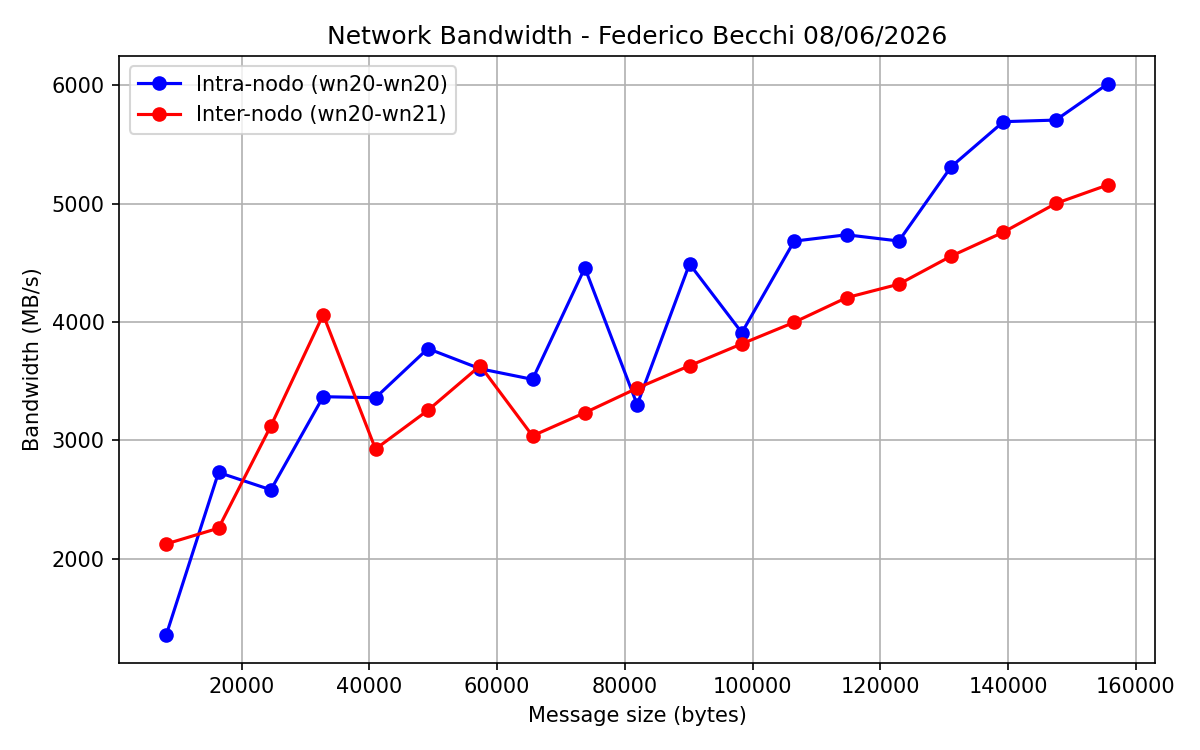
\includegraphics[width=0.7\textwidth]{Cluster/band.png}
  \caption{Network/Cluster/band.png}
\end{figure}

\begin{figure}[H]
  \centering
  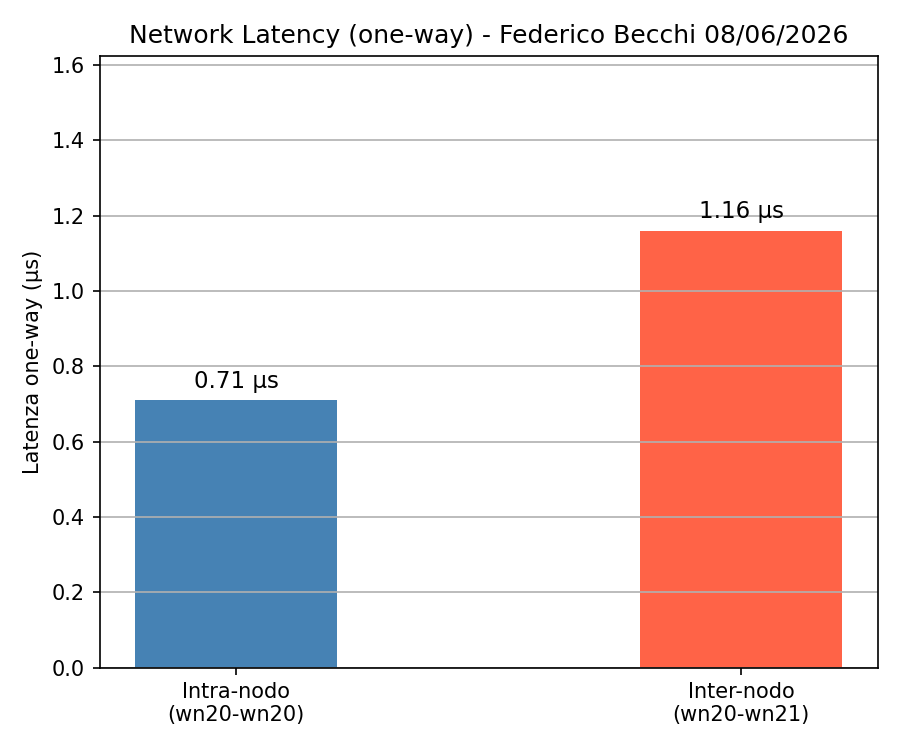
\includegraphics[width=0.7\textwidth]{Cluster/lat.png}
  \caption{Network/Cluster/lat.png}
\end{figure}

\subsection*{Considerazioni}

Sul cluster i test inter-nodo vengono eseguiti attraverso Omnipath quindi ci si aspettano i risultati di latenza e larghezza di banda piu' veloci rispetto al PC, in cui la rete cluster viene simulata attraverso due container docker.
Rispettivamente i test di banda e latenza sono equivalenti.

\end{document}
